{\color{secblue}\subsection{Component View}}
\begin{figure}[H]
    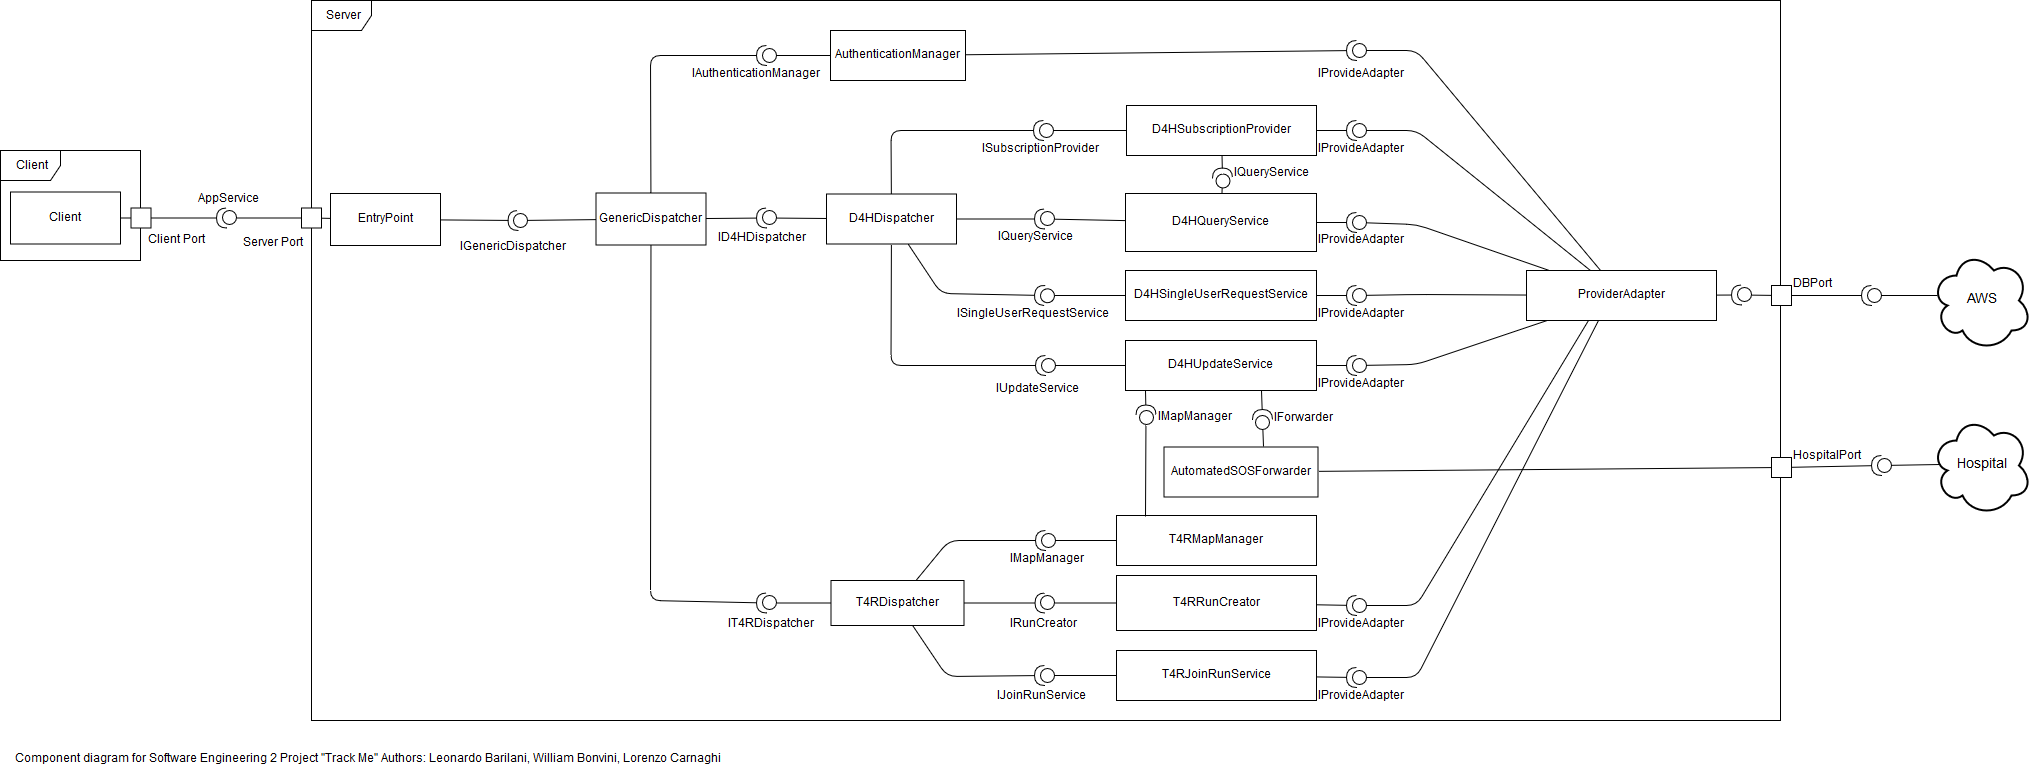
\includegraphics[width=\linewidth, keepaspectratio]{./Images/component_diagram.png}
    \centering
    \caption{Component View of the TrackMe Management Server}
    \label{fig:depview}
  \end{figure}
The components present in the system are the following:
\begin{itemize}
\item Entry Point: this component takes care of receiving all the packets from the clients. It performs some validation checks on the arriving packets. If the packet contains readable and correctly formatted data it is forwarded to Generic Dispatcher;
\item Generic Dispatcher: this component takes care of properly sorting incoming data. Every packet with no exception is passed to Authentication Manager that validates the packet. After validation the Generic Dispatcher reads the type of the packet and it forwards it to the correct component. A packet can be of 3 types:
\begin{itemize}
\item User packet: forwarded to Authentication Manager, this type of packet contains information about registration, login and account management of a user (changing credentials, ecc.);
\item D4H packet: forwarded to D4HDispatcher, this type of packet contains raw data from the users gathered through their smartwatches and smartphones or information about queries;
\item T4R packet: forwarded to T4RDispatcher, this type of packet contains data used to create, manage, join and spectate runs.
\end{itemize}
\item Authentication Manager: this component is used to manage users and third parties credentials and validate incoming packages;
\item D4H Dispatcher: this component analyzes the incoming packet and forwards it to the correct component. A packet can be of 4 types:
\begin{itemize}
\item Subscription packet: forwarded to D4H Subscription Provider, this packet contains information about creating, managing and deleting subscriptions created by third parties users;
\item Query packet: forwarded to D4H Query Service, this packet contains information about executing a query;
\item Single User Request packet: forwarded to D4H Single User Request Service, this packet contains information about a third party user requesting the access to a single user's data;
\item Update packet: forwarded to D4H Update Service, this packet contains information about new raw data gathered from a user's smartwatch or similar device.
\end{itemize}
\item D4H Subscription Provider: this component manages information about creating, managing and deleting subscriptions created by the third parties users. It manages them in the database and also uses the D4H Query Service to perform them;
\item D4H Query Service: this component manages all the queries performed on the raw data collected. It executes them and then decides if they can be deployed or not (i.e. not returning results with less than 1000 records if the query was not about a single user);
\item D4H Single User Request Service: this component manages the interaction between third parties that can request the access to a single user's data and single users that can accept or reject requests. This component memorizes the request in the database;
\item D4H Update Service: this component receives all the new data gathered from users. In order to decide what to do with the new data, the component has to analyze the packet and see what services the user is using:
\begin{itemize}
\item If the packet is marked with the D4H service, then the data contained in the packet is stored in the database;
\item If the packet is marked with the AutomatedSOS service, then the data is sent to the AutomatedSOS Forwarder component;
\item If the packet is marked with the T4R service, then the data is sent to the T4R Map Manager.
\end{itemize}
Note that a packet can be marked with all the 3 services at the same time. This means that a packet can be copied up to 3 times.
\item AutomatedSOS Forwarder: this component analyzes all the packets that it receives and if a packet is marked as "Emergency packet", it starts the procedure that calls the most suitable hospital for the client needs;
\item T4R Dispatcher: this component analyzes the incoming packet and it forwards it to the correct component. A packet can be of 3 types:
\begin{itemize}
\item Map packet: forwarded to T4R Map Manager, this packet is a request for an update of all the positions of the runners for a given run;
\item Create packet: forwarded to T4R Run Creator, this packet contains information about creating a new run;
\item Join packet: forwarded to T4R Join Run Service, this packet contains information about joining an existing run.
\end{itemize}
\item T4R Map Manager: this component stores all the data needed to show a run in progress, i.e. the current position of all the participants. The D4H Update Service sends the position of all the users of different runs to this component, while the T4R Dispatcher requests all the positions of all the participants of a specific run;
\item T4R Run Creator: this component is used to manage the creation of a new run. When a valid request is made, the new run is stored in the database;
\item T4R Join Run Service: this component manages the joining process of a user to a run as a participant of a run (not as a spectator). If the request is valid, then a new participant is added to the requested run;
\item Provider Adapter: this component job is to act as an intermediary between the TrackMe's components that utilize AWS and AWS itself.
\end{itemize}